\documentclass[conference]{IEEEtran}
\IEEEoverridecommandlockouts
\usepackage[T1]{fontenc}
\usepackage{amsmath,amssymb}
\usepackage{graphicx}
\usepackage{booktabs}
\usepackage{xcolor}
\usepackage{tikz}
\usetikzlibrary{positioning,arrows.meta,fit,calc,backgrounds}
\usepackage{pgfplots}
\pgfplotsset{compat=1.18}
\usepackage{url}
\usepackage[hidelinks]{hyperref}

\definecolor{cdmg}{HTML}{D03B3B}
\definecolor{cfault}{HTML}{EB6834}
\definecolor{cenv}{HTML}{2A78D6}
\definecolor{cbase}{HTML}{8A8F98}
\definecolor{cbox}{HTML}{065A82}

\begin{document}

\title{Damage, Weather, or a Broken Sensor? Sequential Alarm Attribution with a False-Alarm Guarantee for Software-Defined AIoT Structural Health Monitoring}

\author{
\IEEEauthorblockN{Hardik Grover\IEEEauthorrefmark{1}, Advait Anand, Akash Kumar, Yograj and Dr.\ P.\ Saravanan}
\IEEEauthorblockA{Department of Computing Technologies, SRM Institute of Science and Technology\\
Kattankulathur Campus, India\\
\IEEEauthorrefmark{1}Corresponding author: hg7243@srmist.edu.in}
}

\maketitle

\begin{abstract}
Data-driven structural health monitoring (SHM) systems usually score each measurement window independently and report every anomaly as possible damage. In a continuously running AIoT deployment this design fails in two ways. First, per-window error rates become hundreds of false alarms per year: even a calibrated 5\,\% per-window rate means about 440 false alarms per year at one window per hour. Second, alarms caused by environmental variation or by faulty IoT sensors cannot be told apart from real damage. We propose ShiftGuard, a monitoring framework with four components: (i)~a self-supervised masked-sensor model that predicts each sensor from the rest of the network and temperature; (ii)~a mask-and-impute step that isolates any single faulty sensor and fills in lost packets; (iii)~temperature-localised conformal p-values that feed three families of conformal e-detectors (CUSUM-type test martingales) for the structure, each sensor and the environment; and (iv)~a conformal severity stage that reports damage severity as a prediction set. Each alarm carries a sequential guarantee, namely that the expected time to a false alarm is at least a chosen threshold, and is attributed to structural damage, unprecedented environmental conditions or a specific faulty sensor. The sensing layer is fully software-defined: virtual MQTT sensor nodes replay a bridge model and the Z24 benchmark through a fault injector, which gives exact ground truth for sensor faults that physical deployments cannot provide. Over a simulated monitoring year with a record cold snap, five types of IoT sensor fault and progressive damage, ShiftGuard reduces false-alarm episodes from 315 to about 8 (and false-alarm hours from 347 to 26) compared with a per-window conformal autoencoder baseline, detects moderate damage within 4\,h, attributes 94\,\% of sensor-fault hours to the correct sensor without labelling any of them as damage, and never labels the cold snap as damage. On the real Z24 bridge recordings it keeps false alarms about 40$\times$ below the baseline (10 vs.\ 391 hours) and detects severe damage, but misses the moderate damage stage.
\end{abstract}

\begin{IEEEkeywords}
Structural health monitoring, AIoT, conformal prediction, test martingales, e-values, sensor fault isolation, environmental variability, Z24 bridge.
\end{IEEEkeywords}

\section{Introduction}
Bridges and buildings degrade silently, through ageing, weather and repeated loading, and damage often develops inside materials that look fine from the outside. Manual inspection is periodic, expensive and subjective, so early-stage damage that appears between inspection cycles can go unnoticed. IoT sensing combined with artificial intelligence (AIoT) promises continuous, automated monitoring, and the literature on IoT-based SHM has grown rapidly over the last decade~\cite{deng2023,rahita2024,li2025}.

Three gaps limit how such systems behave once they run continuously.

\textbf{Gap 1 -- sequential guarantees.} SHM models report accuracy or F1-score on a test set, or at best a per-window calibrated error rate obtained with conformal prediction~\cite{angelopoulos2023}. Monitoring, however, is a sequential problem. With $N$ windows per year, a per-window guarantee $\alpha$ compounds into $N\alpha$ false alarms, and operators stop trusting the system.

\textbf{Gap 2 -- attribution.} A deviation from the healthy baseline has three common causes: structural damage; environmental and operational variation, for example the jump in Z24's natural frequencies when the deck freezes~\cite{peeters2001}; and IoT sensor faults such as drift, noise, dropout, spikes and saturation. Most prior work treats these separately: temperature compensation and sensor-fault isolation (e.g.\ FS-LSTM~\cite{li2021fslstm} and stacked-GRU frameworks~\cite{liu2022sgru}) are separate pipelines, and none comes with a statistical alarm guarantee.

\textbf{Gap 3 -- validation.} Physical deployments cannot provide ground truth for which sensor failed, or when.

The main contributions of this work are:
\begin{enumerate}
\item A masked-sensor healthy-behaviour model whose residuals separate \emph{local} inconsistency (a sensor fault) from \emph{regional} inconsistency (damage). Its mask-and-impute step also repairs lost packets.
\item The first use, to our knowledge, of conformal e-detectors (CUSUM-type conformal test martingales) for SHM alarms. The guarantee is on the expected time to a false alarm, and temperature-localised conformal calibration handles the seasonal covariate shift.
\item A three-way attribution rule (damage / environment / sensor~$i$) together with conformal severity sets.
\item A software-defined AIoT testbed (MQTT virtual nodes, edge monitor, dashboard, an interactive browser digital twin and Node-RED alerts) with a fault-injection protocol that gives exact ground truth.
\end{enumerate}

\section{Related Work}
\subsection{IoT-Based SHM}
Surveys and bibliometric studies document the range of IoT sensors and data-driven methods used for civil structures~\cite{deng2023,rahita2024,li2025,anjali2025}, but they do not propose a deployable alarm logic. AIoT architectures that couple wireless sensing with AI-based interpretation have been validated on aerospace structural testing~\cite{venegas2025}, and edge-computing prototypes run lightweight classifiers such as MobileNetV2 with multi-sensor fusion on laboratory bridges~\cite{wang2025}.

\subsection{Deep Learning on the Z24 Benchmark}
Z24 is the standard benchmark for vibration-based damage detection~\cite{z24}. WaveNet and MiniRocket feature extractors deployed at the edge reach 99.65\,\% accuracy on five-class Z24 classification~\cite{dabbous2024}. A WaveNet model trained on UAV-mounted accelerometer data predicts damage severity and location~\cite{turkomany2025}. A conditional GAN generates synthetic Z24 vibration signals for damage detection and digital twinning~\cite{impraimakis2025}, and a TCN-GAT autoencoder trained only on healthy data detects damage on Z24 and the Old Ada Bridge~\cite{ni2025}. A hybrid convolutional autoencoder with deep SVDD achieves an F1-score of 98.46\,\% on an in-situ truss bridge~\cite{park2025}, and transformer-based masked autoencoders have been proposed as foundation models for SHM~\cite{benfenati2024}. All of these methods make per-window decisions and do not attribute alarms to a cause.

\subsection{Sensor Fault vs.\ Damage}
Kullaa~\cite{kullaa2011} separates sensor faults, structural damage and environmental or operational effects with a statistical model of the sensor network, which is the closest problem setting to ours; its decisions, however, are made window by window, without a guarantee on the false-alarm rate over time. FS-LSTM-based isolation~\cite{li2021fslstm} and stacked-GRU isolation in noisy environments~\cite{liu2022sgru} distinguish sensor faults from structural damage with separate deep classifiers and assume normal environmental conditions.

\subsection{Environmental Variability}
The temperature effect is usually removed by regression, principal component analysis or cointegration before damage detection, in a separate pre-processing step~\cite{peeters2001}.

\subsection{Conformal Prediction and Sequential Testing}
Conformal prediction provides distribution-free, finite-sample coverage guarantees~\cite{angelopoulos2023}. Conformal test martingales extend it to change-point detection~\cite{vovk2021}, e-detectors give a nonparametric framework for sequential change detection~\cite{shin2023}, and WATCH uses weighted-conformal martingales to monitor deployed AI systems~\cite{prinster2025}. None of these has been applied to SHM.

\section{System Architecture}
ShiftGuard runs on a software-defined AIoT stack (Fig.~\ref{fig:arch}).

\textbf{Virtual sensing layer.} Eight accelerometer nodes and one temperature node publish 20\,s windows (100\,Hz) over MQTT once per hour. The source is either an 8-DOF bridge model (first mode about 4\,Hz, with Z24-like stiffening below 0\,\textdegree C) or Z24 recordings~\cite{z24,z24hf} replayed with a temperature warp. A fault injector applies gain, drift, noise, spike, dropout and clipping faults. A Wokwi ESP32\,+\,DHT22 node can override the temperature.

\textbf{Edge analytics.} ShiftGuard (Section~\ref{sec:method}) reassembles each window from the MQTT packets, imputes lost packets and updates all ten detectors in a median of 4.9\,ms per window (p95 9.6\,ms) on a laptop with an Intel Core i5-13420H CPU and 16\,GB RAM (Python~3.13), measured over the live pipeline with the ridge model and including feature extraction.

\textbf{Application layer.} Results are stored in SQLite and shown on a Streamlit dashboard. A browser digital twin connects to the broker over MQTT-over-WebSocket: the deck is animated from the live accelerometer windows, and faults, weather and damage are injected by clicking on the model. A Node-RED flow e-mails damage and sensor-fault alerts (including a severity escalation), while weather alerts only go to the log.

\textbf{Fault tolerance.} Crashed components are restarted by a supervisor and the edge monitor resumes its store. Every MQTT client reconnects with back-off and re-subscribes. Windows are processed in strict sequence order, with late packets imputed, and a restarted sensor network is detected and appended to the history. These behaviours are covered by an automated multi-process test with 20\,\% packet loss and a sensor-network restart.

\begin{figure*}[t]
\centering
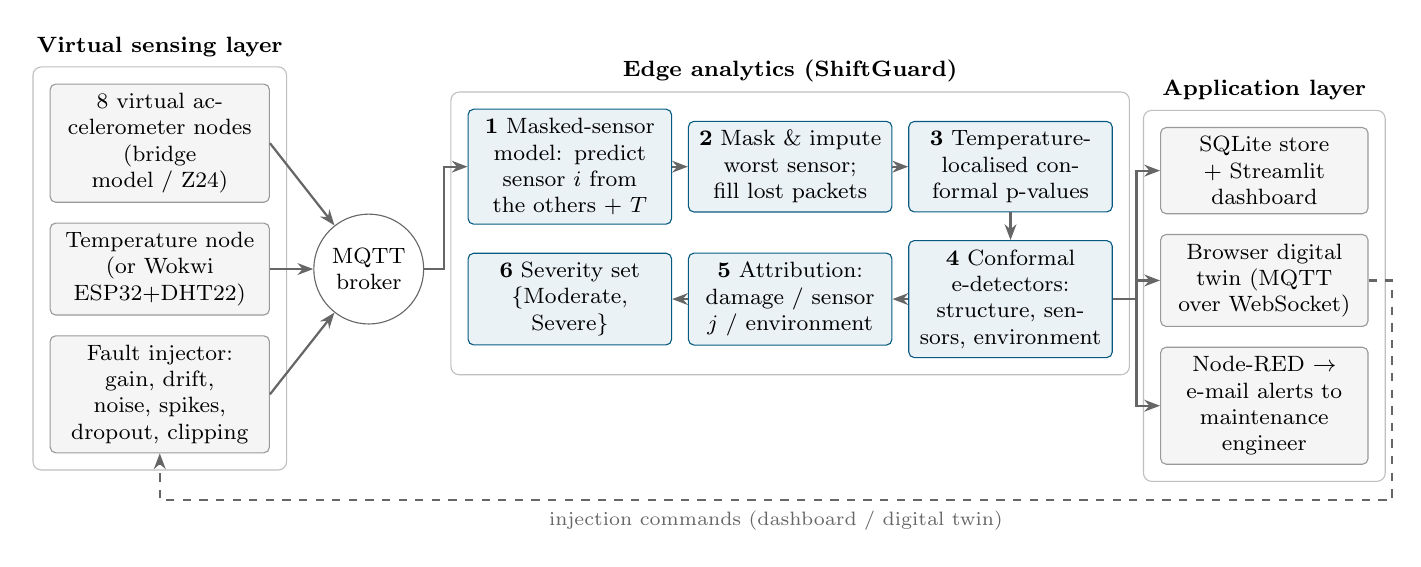
\begin{tikzpicture}[
  font=\footnotesize,
  layer/.style={draw=black!25, rounded corners=3pt, inner sep=6pt},
  src/.style={draw=black!40, fill=black!4, rounded corners=2pt, align=center, text width=2.55cm, minimum height=0.95cm},
  stage/.style={draw=cbox, fill=cbox!8, rounded corners=2pt, align=center, text width=2.35cm, minimum height=1.05cm},
  app/.style={draw=black!40, fill=black!4, rounded corners=2pt, align=center, text width=2.4cm, minimum height=0.95cm},
  arr/.style={-{Stealth[length=2mm]}, thick, black!60}]
\node[src] (acc) {8 virtual accelerometer nodes\\(bridge model / Z24)};
\node[src, below=0.25cm of acc] (temp) {Temperature node\\(or Wokwi ESP32+DHT22)};
\node[src, below=0.25cm of temp] (inj) {Fault injector: gain, drift, noise, spikes, dropout, clipping};
\node[draw=black!60, fill=white, circle, minimum size=1.2cm, align=center, right=0.55cm of temp] (mq) {MQTT\\broker};
\node[stage,right=0.55cm of mq, yshift=1.3cm] (s1) {\textbf{1} Masked-sensor model: predict sensor $i$ from the others + $T$};
\node[stage,right=0.2cm of s1] (s2) {\textbf{2} Mask \& impute worst sensor; fill lost packets};
\node[stage,right=0.2cm of s2] (s3) {\textbf{3} Temperature-localised conformal p-values};
\node[stage,below=0.35cm of s3] (s4) {\textbf{4} Conformal e-detectors: structure, sensors, environment};
\node[stage,left=0.2cm of s4] (s5) {\textbf{5} Attribution: damage / sensor $j$ / environment};
\node[stage,left=0.2cm of s5] (s6) {\textbf{6} Severity set\\\{Moderate, Severe\}};
\node[app, right=0.6cm of s3, yshift=-0.05cm] (db) {SQLite store + Streamlit dashboard};
\node[app, below=0.25cm of db] (twin) {Browser digital twin (MQTT over WebSocket)};
\node[app, below=0.25cm of twin] (nr) {Node-RED $\rightarrow$\\e-mail alerts to\\maintenance engineer};
\begin{scope}[on background layer]
\node[layer, fit=(acc)(temp)(inj), label={[font=\footnotesize\bfseries]above:Virtual sensing layer}] {};
\node[layer, fit=(s1)(s2)(s3)(s4)(s5)(s6), label={[font=\footnotesize\bfseries]above:Edge analytics (ShiftGuard)}] {};
\node[layer, fit=(db)(twin)(nr), label={[font=\footnotesize\bfseries]above:Application layer}] {};
\end{scope}
\draw[arr] (acc.east) -- (mq);
\draw[arr] (temp.east) -- (mq);
\draw[arr] (inj.east) -- (mq);
\draw[arr] (mq.east) -- ++(0.25,0) |- (s1.west);
\draw[arr] (s1) -- (s2); \draw[arr] (s2) -- (s3); \draw[arr] (s3) -- (s4);
\draw[arr] (s4) -- (s5); \draw[arr] (s5) -- (s6);
\draw[arr] (s4.east) -- ++(0.3,0) |- (db.west);
\draw[arr] (s4.east) -- ++(0.3,0) |- (twin.west);
\draw[arr] (s4.east) -- ++(0.3,0) |- (nr.west);
\coordinate (low) at ($(nr.south)+(0,-0.45)$);
\draw[arr, dashed] (twin.east) -- ++(0.3,0) coordinate (tr) -- (tr |- low) -- node[pos=0.5, below, font=\scriptsize] {injection commands (dashboard / digital twin)} (low -| inj.south) -- (inj.south);
\end{tikzpicture}
\caption{Software-defined AIoT architecture of ShiftGuard. Virtual sensor nodes publish windows over MQTT; the edge monitor runs the six-step pipeline of Section~\ref{sec:method}; results feed the dashboard, the digital twin and Node-RED e-mail alerts.}
\label{fig:arch}
\end{figure*}

\section{Proposed Methodology}\label{sec:method}
\subsection{Features}
Each window gives, for each sensor $i$, a vector of $B=16$ log band powers $x_i\in\mathbb{R}^B$ (1--30\,Hz, Welch). The excitation level is removed by subtracting the median over sensors of each sensor's mean log power, so one faulty channel cannot shift the features of the others.

\subsection{Masked-Sensor Model}
A network $f_\theta$ is trained only on healthy data to predict each sensor from the others:
\begin{equation}
\hat{x}_i = f_\theta\big(x_{-i},\, e_i,\, \phi(T)\big),
\end{equation}
where $x_{-i}$ is the window with sensor $i$ masked, $e_i$ is a one-hot sensor index and $\phi(T)$ is a temperature basis that includes a freezing branch. Training randomly masks sensors, so the model is self-supervised. The sensor score is
\begin{equation}
s_i = \frac{1}{B}\left\lVert \frac{x_i-\hat{x}_i}{\sigma_i} \right\rVert^2,
\end{equation}
where $\sigma_i\in\mathbb{R}^B$ is the per-band standard deviation of sensor $i$'s residuals on the healthy fitting data, and the division is element-wise.

\subsection{Mask-and-Impute}
Let $j^*=\arg\max_i s_i$. We replace $x_{j^*}$ by $\hat{x}_{j^*}$, recompute the other sensors' scores $s'_i$, and define the structure score
\begin{equation}
G = \operatorname*{mean}_{i\neq j^*} s'_i .
\end{equation}
A faulty sensor then leaves $G$ unchanged, while damage raises it. The per-sensor detectors use the same masked scores: $\tilde{s}_{j^*}=s_{j^*}$ and $\tilde{s}_i=s'_i$ for $i\neq j^*$. Without this, a faulty sensor also inflates the residuals of the neighbours that are predicted from it; their detectors then accumulate evidence, and when the fault clears the alarm is passed on to a neighbour. Lost packets are imputed the same way: features are computed from the received channels only, and each missing sensor is predicted from the others.

\subsection{Temperature-Localised Conformal p-Values}
For a score $s$ observed at temperature $T$, $s$ is ranked among the $k=400$ calibration scores $c$ recorded at the temperatures closest to $T$:
\begin{equation}
p = \frac{\#\{c>s\} + U\big(\#\{c=s\}+1\big)}{k+1},\quad U\sim\mathcal{U}(0,1).
\end{equation}
This removes the dependence of model error on temperature, which is a benign covariate shift.

\subsection{Conformal e-Detectors}
Each p-value becomes an e-value through a mixture of power calibrators,
\begin{equation}
e = \frac{1}{|E|}\sum_{\varepsilon\in E}\varepsilon\,p^{\varepsilon-1},\qquad \mathbb{E}[e]=1 \text{ under the null.}
\end{equation}
The detector state is updated as
\begin{equation}
M_t = e_t \max(M_{t-1}, 1),
\end{equation}
and raises an alarm when $M_t\geq c$. If the p-values are i.i.d.\ uniform (no change), $\mathbb{E}[\tau_{\text{false}}]\geq c$. We use $c=10^4$ windows, about 14 months at one window per hour. Three families of detectors run in parallel: one for the structure (on $G$); one for each sensor (on $\tilde{s}_i$, with threshold $Nc$, a Bonferroni correction); and one for the environment ($k$-NN novelty of $T$ against the calibration temperatures). The detector state is capped at $10c$ so that it recovers after a condition ends; the cap can only delay an alarm, so it does not weaken the guarantee.

\subsection{Attribution}
Each window is labelled as follows. \textsc{Environment}: an alarm fires while the environment detector is also in alarm; the conditions have never been seen before, so the alarm is held at low confidence. \textsc{Structural damage}: otherwise, the structure detector is in alarm. \textsc{Sensor fault} $j$: only a sensor detector is in alarm.

\subsection{Severity}
After a damage alarm, a logistic model on $\log s$ outputs a split-conformal prediction set over \{Moderate, Severe\} with at least 90\,\% coverage. It is trained on damage at random locations, so the test location is never seen in training.

\section{Experimental Setup}
\subsection{Monitoring Scenario}
The model is trained on one healthy year, with alternate days used for fitting and calibration. It then monitors a second year containing a cold snap 9\,\textdegree C below the seasonal profile (days 15--22); drift on S3 (days 120--134); noise on S6 (days 200--204); dropout on S1 (days 260--262); spikes on S4 (days 285--288); clipping on S7 (days 300--303); and moderate damage (10\,\% stiffness loss, days 330--348) followed by severe damage (25\,\%, days 348--365). One extra healthy-only year checks validity. All results are averaged over 3 random seeds.

\subsection{Baselines and Ablations}
The baseline is an autoencoder-style score (PCA reconstruction error on all features) with a per-window split-conformal threshold at $\alpha=5\,\%$ and $\alpha=0.1\,\%$; this is the pipeline from our earlier design. Five ablations each remove one component: evidence accumulation (the ShiftGuard score with a per-window conformal decision at 5\,\%), masking, temperature-localised calibration (replaced by global calibration), temperature conditioning, and the environment monitor.

\subsection{Metrics}
We report false-alarm hours and episodes on healthy hours; damage detection delay and recall; the fraction of fault hours attributed to the correct sensor; the fraction of fault and cold-snap hours mislabelled as damage; severity-set coverage; and the empirical false-alarm rate on the healthy-only year.

\newcommand{\rowh}{Method & FA h & FA ep. & Delay (h) & Recall & Fault $\checkmark$ & Fault$\to$dmg & Cold$\to$dmg \\}
\begin{table*}[t]
\centering
\caption{Simulated monitoring year, masked-sensor neural model (MLP). Mean of 3 seeds. FA = false alarms on healthy hours; Fault $\checkmark$ = fault hours attributed to the correct sensor; Fault$\to$dmg / Cold$\to$dmg = fault / cold-snap hours labelled as damage.}
\label{tab:mlp}
\begin{tabular}{lrrrrrrr}
\toprule
\rowh
\midrule
ShiftGuard (proposed) & \textbf{26} & 7.7 & 3.7 & 98.7\% & 93.6\% & \textbf{0.0\%} & \textbf{0.0\%} \\
Per-window AE + conformal 5\% & 347 & 314.7 & 4 & 67.6\% & 0.0\% & 86.1\% & 36.1\% \\
Per-window AE + conformal 0.1\% & 7.7 & 3 & 326.3 & 43.8\% & 0.0\% & 70.3\% & 17.3\% \\
Ablation: per-window conformal 5\% (no e-detector) & 351 & 328 & 0 & 86.7\% & 0.0\% & 9.2\% & 31.9\% \\
Ablation: no sensor masking & 40.7 & 7.3 & 3.7 & 98.7\% & 3.4\% & 90.9\% & 0.2\% \\
Ablation: global (not temperature-localised) calibration & 106 & 16.7 & 7 & 98.3\% & 93.9\% & 0.0\% & 6.3\% \\
Ablation: no temperature conditioning & 28.7 & 9.3 & 4.7 & 98.6\% & 93.8\% & 0.1\% & 0.0\% \\
Ablation: no environment monitor & 26.7 & 7.7 & 4 & 99.5\% & 93.5\% & 0.0\% & 33.5\% \\
\bottomrule
\end{tabular}
\end{table*}

\begin{table*}[t]
\centering
\caption{The same experiment with the linear cross-sensor model (ridge). Mean of 3 seeds.}
\label{tab:ridge}
\begin{tabular}{lrrrrrrr}
\toprule
\rowh
\midrule
ShiftGuard (proposed) & \textbf{23.3} & 6.7 & 2.7 & 98.8\% & 95.7\% & 1.2\% & \textbf{0.0\%} \\
Per-window AE + conformal 5\% & 347 & 314.7 & 4 & 67.6\% & 0.0\% & 86.1\% & 36.1\% \\
Per-window AE + conformal 0.1\% & 7.7 & 3 & 326.3 & 43.8\% & 0.0\% & 70.3\% & 17.3\% \\
Ablation: per-window conformal 5\% (no e-detector) & 377 & 349.7 & 0 & 96.3\% & 0.0\% & 18.3\% & 30.8\% \\
Ablation: no sensor masking & 36.3 & 8.3 & 2.3 & 98.8\% & 1.0\% & 96.4\% & 0.0\% \\
Ablation: global (not temperature-localised) calibration & 64.3 & 13 & 7.3 & 98.3\% & 97.3\% & 0.1\% & 0.6\% \\
Ablation: no temperature conditioning & 26.3 & 7.7 & 2.7 & 98.8\% & 95.7\% & 1.3\% & 0.0\% \\
Ablation: no environment monitor & 24 & 7 & 3 & 99.6\% & 94.9\% & 2.0\% & 33.3\% \\
\bottomrule
\end{tabular}
\end{table*}

\section{Results and Discussion}
\subsection{Simulated Monitoring Year}
Tables~\ref{tab:mlp} and~\ref{tab:ridge} report the simulated year for the neural and the linear variant. Five observations stand out.

\textbf{Accumulating evidence is what removes false alarms.} The per-window decision on the same ShiftGuard score gives about 330--350 false-alarm episodes, against 7--8 for the e-detector (Fig.~\ref{fig:fa}).

\textbf{Masking is what makes fault attribution possible.} Without it, 91--96\,\% of fault hours are called damage, against 0--1\,\% with masking (Fig.~\ref{fig:abl}).

\textbf{Localised calibration} cuts false-alarm hours by about 75\,\% (106\,$\rightarrow$\,26\,h for the MLP, 64\,$\rightarrow$\,23\,h for ridge) and halves detection delay.

\textbf{The environment monitor} is what stops the cold snap being called damage (33\,\%\,$\rightarrow$\,0\,\%).

\textbf{The baselines face a dilemma.} At $\alpha=5\,\%$ the baseline detects damage fast but raises 315 false-alarm episodes. At $\alpha=0.1\,\%$ it misses moderate damage entirely, with a 326\,h delay and 44\,\% recall.

\subsection{Validity of the Guarantee}
On the healthy-only year (3 seeds), ShiftGuard raises 3.3 (MLP) and 2.7 (ridge) false-alarm episodes per year, against 390 for the per-window 5\,\% baseline. The design target is $\mathbb{E}[\text{time to false alarm}]\geq 1.14$ years. Taking into account the per-sensor detectors (a union bound gives $c/2$ overall) and hourly autocorrelation, the realised rate is a few episodes per year: about 100$\times$ fewer than the baseline, but above the nominal bound. Raising $c$ to $10^5$ lengthens the detection delay by about 20\,\% (2.7\,$\rightarrow$\,3.3\,h, ridge, 3 seeds) but removes only about 10\,\% of the false-alarm hours (23.3\,$\rightarrow$\,20.7\,h), so $c=10^4$ is a reasonable operating point.

\begin{figure}[t]
\centering
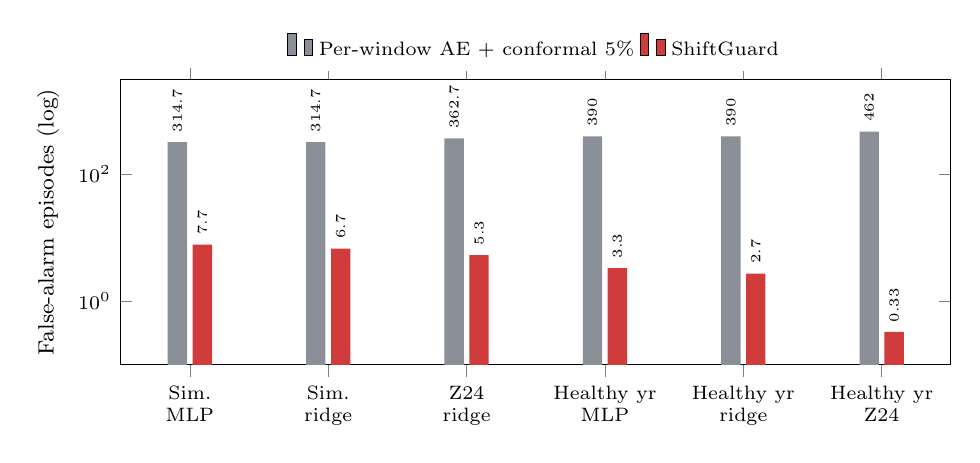
\begin{tikzpicture}
\begin{axis}[
  width=\columnwidth, height=5.2cm,
  ybar, bar width=7pt, ymode=log, log origin=infty,
  ymin=0.1, ymax=3000,
  ylabel={False-alarm episodes (log)}, ylabel style={font=\footnotesize},
  symbolic x coords={SimMLP,SimRidge,Z24Ridge,HyMLP,HyRidge,HyZ24},
  xtick={SimMLP,SimRidge,Z24Ridge,HyMLP,HyRidge,HyZ24},
  xticklabels={{Sim.\\MLP},{Sim.\\ridge},{Z24\\ridge},{Healthy yr\\MLP},{Healthy yr\\ridge},{Healthy yr\\Z24}},
  xticklabel style={font=\scriptsize, align=center},
  yticklabel style={font=\scriptsize},
  nodes near coords, nodes near coords style={font=\tiny, rotate=90, anchor=west},
  point meta=explicit symbolic,
  legend style={font=\scriptsize, at={(0.5,1.03)}, anchor=south, legend columns=2, draw=none},
  enlarge x limits=0.1]
\addplot[fill=cbase, draw=none] coordinates {(SimMLP,314.7)[314.7] (SimRidge,314.7)[314.7] (Z24Ridge,362.7)[362.7] (HyMLP,390)[390] (HyRidge,390)[390] (HyZ24,462)[462]};
\addplot[fill=cdmg, draw=none] coordinates {(SimMLP,7.7)[7.7] (SimRidge,6.7)[6.7] (Z24Ridge,5.3)[5.3] (HyMLP,3.3)[3.3] (HyRidge,2.7)[2.7] (HyZ24,0.33)[0.33]};
\legend{Per-window AE + conformal 5\%, ShiftGuard}
\end{axis}
\end{tikzpicture}
\caption{False-alarm episodes per monitored year: per-window baseline vs.\ ShiftGuard on the simulated year, on Z24, and on healthy-only validity years (values from Tables~\ref{tab:mlp}--\ref{tab:z24}).}
\label{fig:fa}
\end{figure}

\begin{figure}[t]
\centering
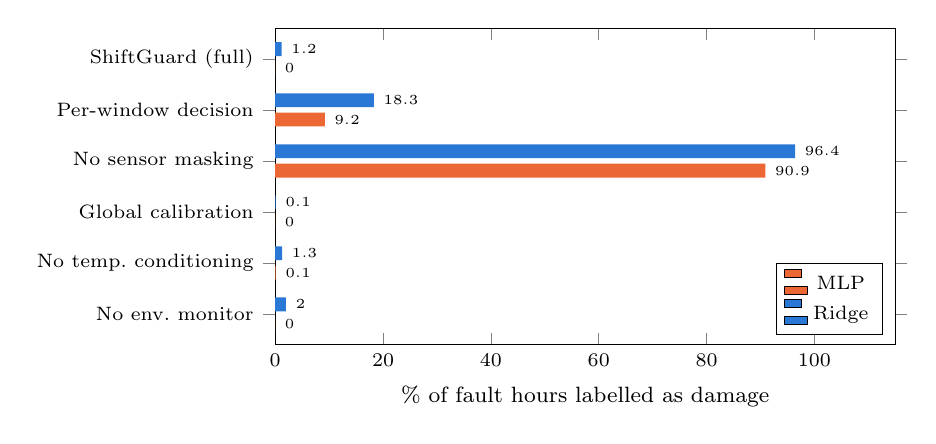
\begin{tikzpicture}
\begin{axis}[
  width=0.78\columnwidth, height=5.6cm,
  xbar, bar width=5pt, xmin=0, xmax=115,
  xlabel={\% of fault hours labelled as damage}, xlabel style={font=\footnotesize},
  symbolic y coords={NoEnv,NoTemp,Global,NoMask,PerWindow,Full},
  ytick={NoEnv,NoTemp,Global,NoMask,PerWindow,Full},
  yticklabels={No env.\ monitor, No temp.\ conditioning, Global calibration, No sensor masking, Per-window decision, ShiftGuard (full)},
  yticklabel style={font=\scriptsize}, xticklabel style={font=\scriptsize},
  nodes near coords, nodes near coords style={font=\tiny},
  legend style={font=\scriptsize, at={(0.98,0.03)}, anchor=south east},
  enlarge y limits=0.12]
\addplot[fill=cfault, draw=none] coordinates {(0,Full) (9.2,PerWindow) (90.9,NoMask) (0,Global) (0.1,NoTemp) (0,NoEnv)};
\addplot[fill=cenv, draw=none] coordinates {(1.2,Full) (18.3,PerWindow) (96.4,NoMask) (0.1,Global) (1.3,NoTemp) (2.0,NoEnv)};
\legend{MLP, Ridge}
\end{axis}
\end{tikzpicture}
\caption{Ablation: share of sensor-fault hours mislabelled as structural damage (Tables~\ref{tab:mlp} and~\ref{tab:ridge}). Removing mask-and-impute turns almost every sensor fault into a false damage alarm.}
\label{fig:abl}
\end{figure}

\subsection{Severity and Localisation}
The conformal severity sets reach 100\,\% (MLP) and 99.7\,\% (ridge) coverage against a 90\,\% target, with an average set size of 1.0. During severe damage, the mean per-sensor residual peaks at S5--S6, where the damage was placed. For ridge the residuals are 23.7 and 24.1 against at most 9.3 elsewhere; for the MLP the peak is less sharp (S5\,=\,11.0, S4\,=\,9.2).

\begin{table*}[t]
\centering
\caption{The same protocol on the real Z24 recordings (ridge model, mean of 3 seeds). The last row uses the masked-sensor MLP.}
\label{tab:z24}
\begin{tabular}{lrrrrrrr}
\toprule
\rowh
\midrule
ShiftGuard (proposed) & \textbf{10.3} & 5.3 & 494 & 23.5\% & 46.5\% & 0.3\% & \textbf{0.0\%} \\
Per-window AE + conformal 5\% & 391.3 & 362.7 & 70.7 & 10.4\% & 0.0\% & 23.0\% & 16.5\% \\
Per-window AE + conformal 0.1\% & 12.7 & 12.3 & 94.3 & 1.5\% & 0.0\% & 12.6\% & 2.4\% \\
Ablation: per-window conformal 5\% (no e-detector) & 367.3 & 343.3 & 68 & 16.0\% & 0.0\% & 8.6\% & 9.7\% \\
Ablation: no sensor masking & 16.7 & 7 & 37 & 30.6\% & 4.8\% & 41.8\% & 0.0\% \\
Ablation: global (not temperature-localised) calibration & 11.7 & 6.7 & 493.3 & 23.6\% & 45.7\% & 2.0\% & 0.0\% \\
Ablation: no temperature conditioning & 10.3 & 5.3 & 494.3 & 23.3\% & 46.2\% & 0.3\% & 0.0\% \\
Ablation: no environment monitor & 10.7 & 5.7 & 492.7 & 25.4\% & 47.9\% & 0.3\% & 3.0\% \\
\midrule
ShiftGuard (MLP) & 12.7 & 5.7 & 494 & 27.3\% & 44.7\% & 0.0\% & 0.0\% \\
\bottomrule
\end{tabular}
\end{table*}

\subsection{Real Z24 Recordings}
The processed Z24 progressive-damage data~\cite{z24,z24hf} has 1530 recordings (17 scenarios $\times$ 9 sensor setups $\times$ 10 segments, 27 channels, 60\,s at 100\,Hz). Scenarios 1--2 are healthy, scenarios 3--7 and 9--11 are moderate damage, and scenarios 12--17 are severe damage; scenario 8 (the new reference after settlement) is excluded. The cross-sensor model needs a fixed sensor layout. With a single setup there are only 20 healthy recordings, and calibration and test windows then come from different recordings, which breaks exchangeability: ShiftGuard raised 795 false-alarm hours in a 120-day pilot run. We therefore use the 8 channels whose RMS level is as stable \emph{between} setups as \emph{within} a setup (channels 1, 2, 3, 9, 13, 17, 18, 19). These behave like the fixed reference sensors of the Z24 campaign, so all 180 healthy recordings can be used; the selection uses healthy recordings only. Healthy recordings are split 50/25/25\,\% into fitting, calibration and the monitored stream, and damaged recordings 40/20/40\,\% into severity training, severity calibration and the stream. The same event schedule as in Section~V is applied: sensor faults are injected into the replayed recordings, and the cold snap is imposed through the temperature warp of Section~III. Table~\ref{tab:z24} reports the results.

\textbf{False alarms carry over from simulation to real data.} ShiftGuard gives 10.3 false-alarm hours (5.3 episodes) against 391 hours (363 episodes) for the per-window baseline. The healthy-only year gives 0.33 false-alarm episodes, against 462 for the baseline.

\textbf{Weather and sensor faults are still not mistaken for damage.} Only 0.3\,\% of fault hours and 0\,\% of cold-snap hours are labelled damage, against 23\,\% and 16.5\,\% for the baseline.

\textbf{Damage detection is the weak point on Z24.} Recall is 23.5\,\% and the first damage alarm comes after about 494\,h, which is 62\,h into the severe stage: the moderate stage (pier settlement, spalling, landslide) is missed on these channels. The baseline is no better (10.4\,\% recall at $\alpha=5\,\%$). The early Z24 damage scenarios change the response of the shared reference channels very little.

\textbf{Fault attribution to the correct sensor drops to 46.5\,\%} (95.7\,\% in simulation), although faults are almost never called damage. Real recordings have weaker cross-sensor redundancy than the 8-DOF model, so a fault on one channel is more often blamed on a neighbour.

\textbf{Severity sets keep their coverage guarantee} (92.4\,\% against a 90\,\% target) but are less sharp (average set size 1.46, against 1.0 in simulation).

With the masked-sensor MLP instead of ridge, ShiftGuard gives 12.7 false-alarm hours, 27.3\,\% damage recall and 2.67 false-alarm episodes in the healthy-only year, with 90.4\,\% severity-set coverage; the conclusions are the same as for ridge.

\subsection{Discussion and Limitations}
Accumulating evidence is what removes false alarms: the ablation that keeps ShiftGuard's score but decides window-by-window is about as noisy as the baseline. Masking is what turns sensor faults from ``damage'' into correctly localised maintenance tickets, and temperature-localised calibration is what keeps the guarantee valid across seasons. Several limitations remain.

\textbf{The guarantee is approximate.} It assumes exchangeable healthy windows, while hourly windows are autocorrelated; the healthy-only year reports how much this matters in practice.

\textbf{Single-fault assumption.} Mask-and-impute removes one sensor per window, so simultaneous faults would need an iterative version. Lost packets are already imputed iteratively, for any number of missing sensors up to half the network.

\textbf{Simulated temperature effect.} The Z24 temperature effect is simulated, because the progressive-damage test has no temperature channel. Long-term Z24 monitoring data~\cite{peeters2001} would allow a fully measured evaluation.

\textbf{Z24 damage sensitivity.} On the 8 shared reference channels, moderate Z24 damage is not detected (Table~\ref{tab:z24}). The alarm guarantee and the attribution of faults and weather hold on real data, but damage sensitivity depends on sensor placement and features. Using the full setup-specific layouts, or modal features instead of band powers, is future work.

\textbf{Model choice.} The linear (ridge) variant localises damage more sharply, while the neural variant is the self-supervised masked model. Both give the same alarm behaviour, so the framework is model-agnostic.

\section{Conclusion}
ShiftGuard reframes SHM alarms as a sequential, attributable decision. It answers \emph{what} changed (the structure, the weather or a sensor) and gives a statistical bound on how often it raises a false alarm. On a simulated monitoring year it cuts false-alarm episodes from 315 to about 8 while detecting moderate damage within 4\,h, and on real Z24 recordings it keeps false alarms about 40$\times$ below a per-window baseline without mistaking weather or sensor faults for damage. The software-defined AIoT testbed makes this evaluation possible with exact ground truth. Future work will improve damage sensitivity on real structures with setup-specific layouts and modal features, and extend mask-and-impute to simultaneous sensor faults.

\section*{Code and Data Availability}
The ShiftGuard code, the software-defined testbed, the experiment scripts and all result files are available from the corresponding author on request. The Z24 recordings are publicly available~\cite{z24,z24hf}.

\begin{thebibliography}{99}
\bibitem{deng2023} H.~Deng and J.~Chen, ``A survey of structural health monitoring advances based on Internet of Things (IoT) sensors,'' \emph{Int. J. Adv. Comput. Sci. Appl.}, vol.~14, no.~10, 2023.
\bibitem{rahita2024} A.~C. Rahita, A.~Zaki, G.~Nugroho, and S.~Yadi, ``Internet of Things (IoT) in structural health monitoring: A decade of research trends,'' IIETA, 2024.
\bibitem{li2025} B.~Li, Y.~Li, and K.~Noman, ``Structural health monitoring: Advanced sensing, diagnostics and prognostics,'' \emph{Sensors}, vol.~25, no.~5, 2025.
\bibitem{venegas2025} P.~Venegas, U.~Virto, I.~Calvo, and O.~Barambones, ``An AIoT architecture for structural testing: Application to a real aerospace component,'' 2025.
\bibitem{anjali2025} P.~Anjali, Y.~Rajesh, T.~Ramesh, P.~Janakiram, and N.~Vasu, ``Structural health monitoring using IoT,'' \emph{Int. J. Res. Publ. Rev.}, vol.~6, no.~11, 2025.
\bibitem{park2025} S.~Park and S.~Kim, ``Hybrid CAE--DSVDD for unsupervised vibration-based damage detection in in-situ steel truss bridge,'' \emph{Struct. Health Monit.}, 2025.
\bibitem{dabbous2024} A.~Dabbous, R.~Berta, M.~Fresta, H.~Ballout, L.~Lazzaroni, and F.~Bellotti, ``Bringing intelligence to the edge for structural health monitoring: The case study of the Z24 bridge,'' \emph{IEEE Open J. Ind. Electron. Soc.}, vol.~5, 2024.
\bibitem{turkomany2025} M.~Turkomany, A.~I. AbdelLatef, and N.~Uddin, ``A novel WaveNet deep learning approach for enhanced bridge damage detection,'' \emph{Appl. Sci.}, vol.~15, no.~22, 2025.
\bibitem{wang2025} Y.~Wang, Z.~Tang, G.~Qian, W.~Xu, X.~Huang, and H.~Fang, ``A prototype of a lightweight structural health monitoring system based on edge computing,'' \emph{Sensors}, vol.~25, no.~18, 2025.
\bibitem{impraimakis2025} M.~Impraimakis and E.~N. Palkanoglou, ``A generative adversarial network optimization method for damage detection and digital twinning: Z24 bridge SHM benchmark validation,'' \emph{Struct. Multidiscip. Optim.}, 2025.
\bibitem{ni2025} Y.~Ni, Q.~Jin, and R.~Hu, ``A novel unsupervised structural damage detection method based on TCN-GAT autoencoder,'' \emph{Sensors}, vol.~25, no.~21, Art. no.~6724, 2025.
\bibitem{angelopoulos2023} A.~N. Angelopoulos and S.~Bates, ``Conformal prediction: A gentle introduction,'' \emph{Found. Trends Mach. Learn.}, vol.~16, no.~4, pp.~494--591, 2023.
\bibitem{z24} KU Leuven / EMPA, ``Z24 bridge structural health monitoring benchmark dataset,'' 1998. [Online]. Available: \url{https://bwk.kuleuven.be/bwm/z24}
\bibitem{vovk2021} V.~Vovk, I.~Petej, I.~Nouretdinov, E.~Ahlberg, L.~Carlsson, and A.~Gammerman, ``Retrain or not retrain: Conformal test martingales for change-point detection,'' in \emph{Proc. COPA}, PMLR, vol.~152, 2021.
\bibitem{shin2023} J.~Shin, A.~Ramdas, and A.~Rinaldo, ``E-detectors: A nonparametric framework for sequential change detection,'' \emph{New England J. Statist. Data Sci.}, 2023 (arXiv:2203.03532).
\bibitem{prinster2025} D.~Prinster, X.~Han, A.~Liu, and S.~Saria, ``WATCH: Adaptive monitoring for AI deployments via weighted-conformal martingales,'' in \emph{Proc. ICML}, 2025.
\bibitem{benfenati2024} L.~Benfenati \emph{et~al.}, ``Foundation models for structural health monitoring,'' arXiv:2404.02944, 2024.
\bibitem{peeters2001} B.~Peeters and G.~De~Roeck, ``One-year monitoring of the Z24-Bridge: Environmental effects versus damage events,'' \emph{Earthquake Eng. Struct. Dyn.}, vol.~30, no.~2, 2001.
\bibitem{li2021fslstm} L.~Li, G.~Liu, L.~Zhang, and Q.~Li, ``FS-LSTM-based sensor fault and structural damage isolation in SHM,'' \emph{IEEE Sensors J.}, vol.~21, no.~3, pp.~3250--3259, 2021, doi: 10.1109/JSEN.2020.3022099.
\bibitem{liu2022sgru} B.~Liu, Q.~Xu, J.~Chen, J.~Li, and M.~Wang, ``A new framework for isolating sensor failures and structural damage in noisy environments based on stacked gated recurrent unit neural networks,'' \emph{Buildings}, vol.~12, no.~8, Art. no.~1286, 2022, doi: 10.3390/buildings12081286.
\bibitem{kullaa2011} J.~Kullaa, ``Distinguishing between sensor fault, structural damage, and environmental or operational effects in structural health monitoring,'' \emph{Mech. Syst. Signal Process.}, vol.~25, no.~8, pp.~2976--2989, 2011, doi: 10.1016/j.ymssp.2011.05.017.
\bibitem{z24hf} T.~Le~Xuan, ``Z24 dataset (processed),'' Hugging Face. [Online]. Available: \url{https://huggingface.co/datasets/thanglexuan/Z24-dataset-processed}
\end{thebibliography}

\end{document}
